\documentclass[12pt]{article}
\usepackage[utf8]{inputenc}
\usepackage[spanish]{babel}
\decimalpoint
\usepackage{amsmath}
\usepackage{amsthm}
\usepackage{amssymb}
\usepackage{graphicx}
\usepackage[margin=0.9in]{geometry}
\usepackage{fancyhdr}
\usepackage[inline]{enumitem}
\usepackage{float}
\usepackage{cancel}
\usepackage{bigints}
\usepackage{color}
\usepackage{xcolor}
\usepackage{listings}
\usepackage{listingsutf8}
\usepackage{algorithm}
\usepackage{tocloft}
\usepackage[none]{hyphenat}
\usepackage{graphicx}
\usepackage{grffile}
\usepackage{tabularx}
\usepackage[nottoc,notlot,notlof]{tocbibind}
\renewcommand{\cftsecleader}{\cftdotfill{\cftdotsep}}
\pagestyle{fancy}
\setlength{\headheight}{15pt} 
\lhead {Administrador de Procesos en Linux y Windows (1)}
\rhead{\thepage}
\lfoot{Sistemas Operativos}
\renewcommand{\footrulewidth}{0.5pt}
\setlength{\parskip}{0.5em}
\newcommand{\ve}[1]{\overrightarrow{#1}}
\newcommand{\abs}[1]{\left\lvert #1 \right\lvert}
\definecolor{pblue}{rgb}{0.13,0.13,1}
\definecolor{pgreen}{rgb}{0,0.5,0}
\definecolor{pred}{rgb}{0.9,0,0}
\definecolor{pgrey}{rgb}{0.46,0.45,0.48}
\lstset{tabsize=1}
\bibliographystyle{IEEEtran}
\usepackage{listings}
\definecolor{dkgreen}{rgb}{0,0.6,0}
\definecolor{gray}{rgb}{0.5,0.5,0.5}
\definecolor{mauve}{rgb}{0.58,0,0.82}

\usepackage{hyperref}
\usepackage{listings}
\lstdefinestyle{customc}{
  belowcaptionskip=1\baselineskip,
  numbers=left,                   % where to put the line-numbers
  numberstyle=\tiny\color{gray},  % the style that is used for the line-numbers
  stepnumber=1,   
  breaklines=true,
  xleftmargin=\parindent,
  language=C,
  showstringspaces=false,
  basicstyle=\footnotesize,
  keywordstyle=\bfseries\color{green!40!black},
  commentstyle=\itshape\color{purple!40!black},
  identifierstyle=\color{blue},
  stringstyle=\color{orange},
}

\lstdefinestyle{customasm}{
  belowcaptionskip=1\baselineskip,
  frame=L,
  xleftmargin=\parindent,
  language=[x86masm]Assembler,
  basicstyle=\footnotesize\ttfamily,
  commentstyle=\itshape\color{purple!40!black},
}

\lstset{escapechar=@,style=customc}
\begin{document}
		\begin{titlepage}
			\begin{center}
				% Upper part of the page. The '~' is needed because \\
				% only works if a paragraph has started.
				\noindent
				\begin{minipage}{0.5\textwidth}
					\begin{flushleft} \large
					
\includegraphics[width=0.3\textwidth]{Imagenes/ipn.png}
					\end{flushleft}
				\end{minipage}%
				\begin{minipage}{0.55\textwidth}
					\begin{flushright} \large
			       	
\includegraphics[width=0.7\textwidth]{Imagenes/escom.png}
					\end{flushright}
				\end{minipage}
				\textsc{\LARGE Instituto Politécnico Nacional}\\[0.5cm]
				\textsc{\Large Escuela Superior de Cómputo}\\[1cm]
				% Title
				{ \huge Práctica No.4 \\[1cm] }
				{\huge Administrador de Procesos en Linux y Windows (1)\\[1cm]}
				{ \Large Unidad de aprendizaje: Sistemas Operativos} \\[1cm]
				{ \Large Grupo: 2CM8 } \\[1cm]
				\noindent
				\begin{minipage}{0.5\textwidth}
					\begin{flushleft} \large
						\emph{Integrantes del equipo:}\\
						\begin{tabular}{ll}
					     Domínguez Morán Joaquín\\
					     Carrillo Balcazar Eduardo Yair\\
					     Ruiz López Luis Carlos\\
					\end{tabular}
					\end{flushleft}
				\end{minipage}%
				\begin{minipage}{0.5\textwidth}
					\begin{flushright} \large
						\emph{Profesor:} \\
						Jorge Cortes Galicia 
					\end{flushright}
				\end{minipage}
				
				\vfill
				% Bottom of the page
				{\large 22 de octubre de 2018}
			\end{center}
		\end{titlepage}
		
\section{Competencias.}
El alumno aprende a familiarizarse con el administrador de procesos del sistema operativo Linux y Windows a través de la creación de nuevos procesos por copia exacta de código y/o por sustitución de código para el desarrollo de aplicaciones concurrentes sencillas.
\section{Desarrollo.}
    \subsection{Linux}
    \begin{enumerate}
        \item Introduzca los siguientes comandos a través de la consola del sistema operativo Linux:
        \begin{itemize}
            \item Ps: proporciona una captura de todos los procesos que se se encuentran actualmente
            \item Ps -fea: proporciona de igual forma los procesos pero ahora proporciona mayor información y además incluye los procesos del sistema.
             \begin{center}
                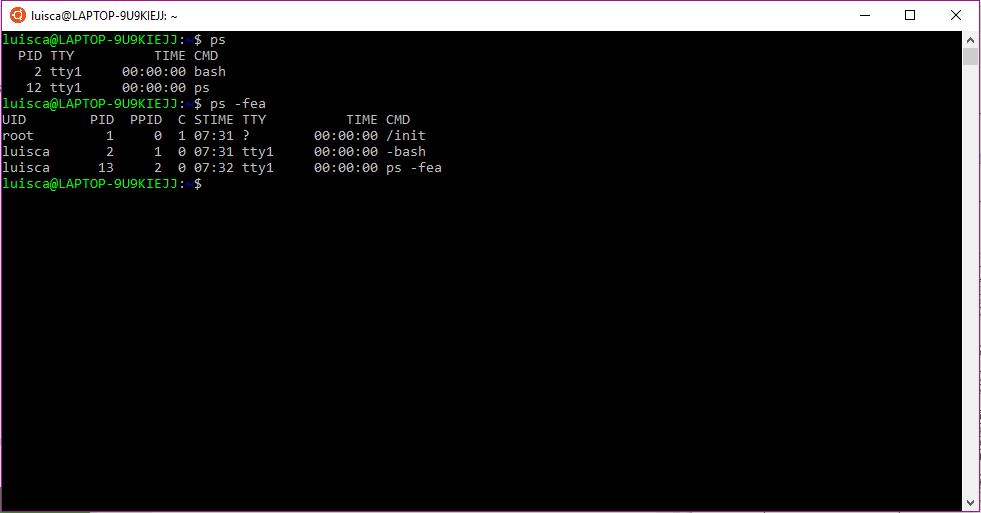
\includegraphics[scale=.55]{Imagenes/Linux/PsPs-fea.PNG}
            \end{center}

        \end{itemize}
        \item A continuación se mencionan los  usos del comando  ps y  las opciones de uso de dicho comando.\\
       \textbf{ps}  Reporta una captura de los procesos actuales.
       
        Algunas de sus opciones son:
        \begin{itemize}
            \item \textbf{-e} Visualiza información sobre "todos" los procesos del sistema.
            \item \textbf{-A} Selecciona todos los procesos, parecido a -e
            \item \textbf{-j} Visualiza información sobre el PGID y SID.
            \item \textbf{-l} Visualiza "mucha" información sobre los procesos (difiere a poner el signo menos delante).
            \item \textbf{-f} Visualiza los parámetros con los que se levantó el proceso.
            \item \textbf{-a} Muestra también los procesos de otros usuarios.
            \item \textbf{-N} Niega el efecto de cualquier opción que se haya especificado.
            \item \textbf{-x} Muestra procesos que no están controlados por ninguna terminal.
            \item \textbf{-u} El usuario visualiza información de los procesos del usuario.
        \end{itemize}
         \begin{center}
                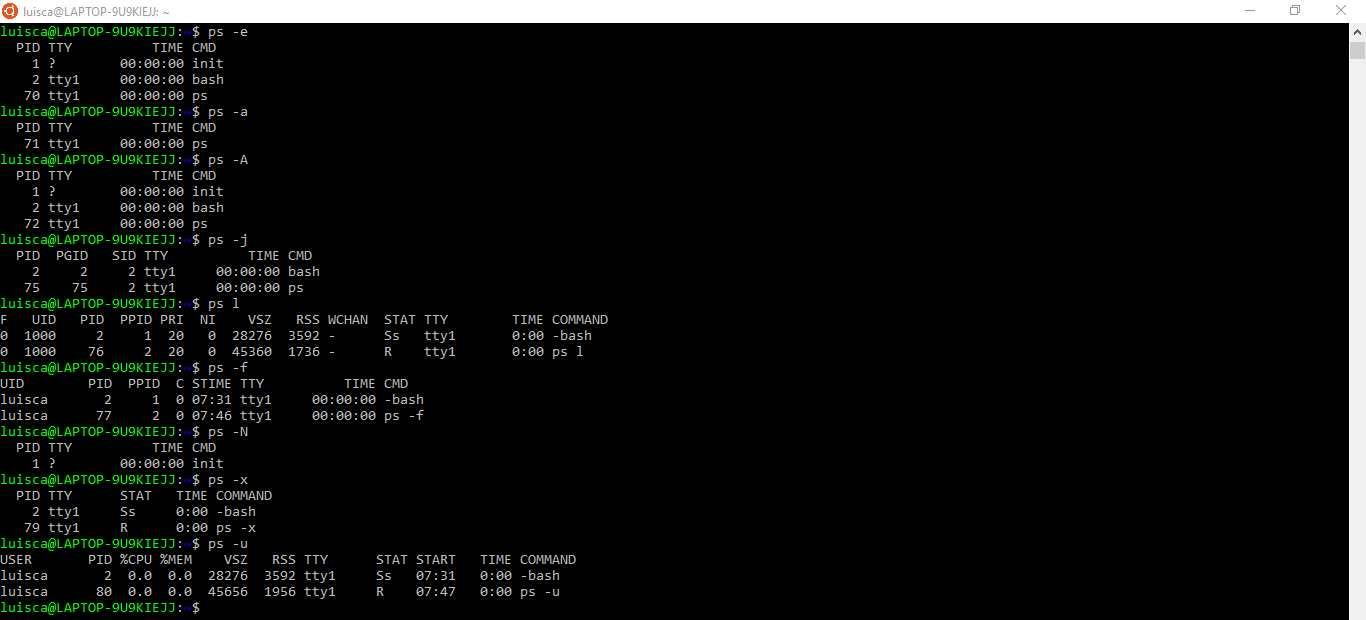
\includegraphics[scale=.45]{Imagenes/Linux/psvariantes.PNG}
            \end{center}
       A continuación se explica el uso de las siguientes llamadas al sistema:
        \begin{itemize}
            \item \textbf{fork():} Crea un proceso hijo. Crea un proceso por copia exacta de código del proceso que lo llama.
            \item \textbf{execv():} Remplaza la imagen del proceso con otra nueva imagen de proceso 
            \item \textbf{getpid():} Regresa el ID del proceso que la llamo
            \item \textbf{getppid():}: Regresa el ID del proceso padre del proceso que llamo la función
            \item \textbf{wait():} La función hace que el proceso espere por la finalización de cualquier hijo y retorna el PID del proceso hijo. El proceso se bloquea hasta que exista un hijo que termine.

        \newpage
        \end{itemize}
        \item Capture, compile y ejecute los dos programas de creación de un nuevo proceso por copia exacta de código que a continuación se muestra. Observe su funcionamiento y experimente con el código.\\
        
            \textbf{Código 1}
            \lstinputlisting{Codigo/Linux/3.1.c}
            \textbf{Código 2}
            \lstinputlisting{Codigo/Linux/3.2.c}
            \newpage
            \textbf{Ejecución de Código 1}
             \begin{center}
                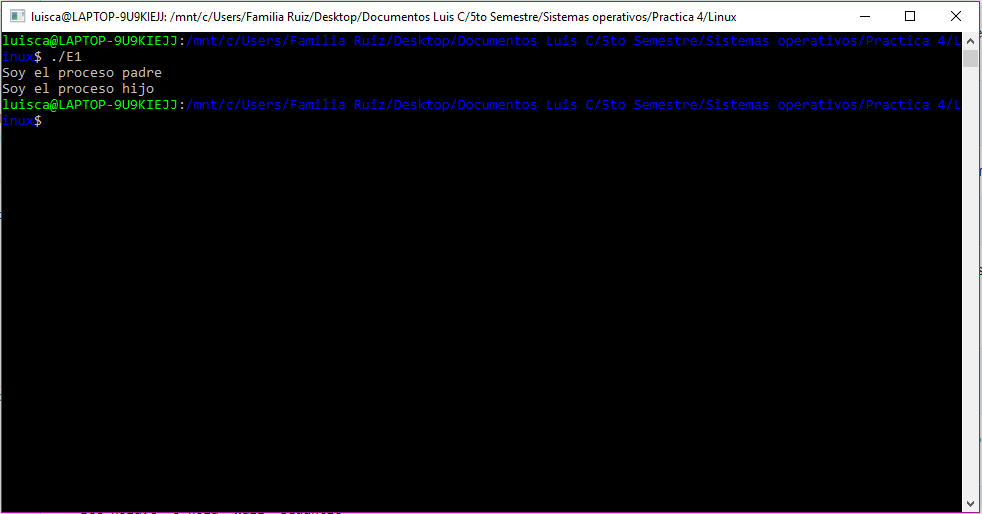
\includegraphics[scale=.5]{Imagenes/Linux/Ejemplo 1.PNG}
            \end{center}
            \textbf{Ejecución de Código 2}
            \begin{center}
                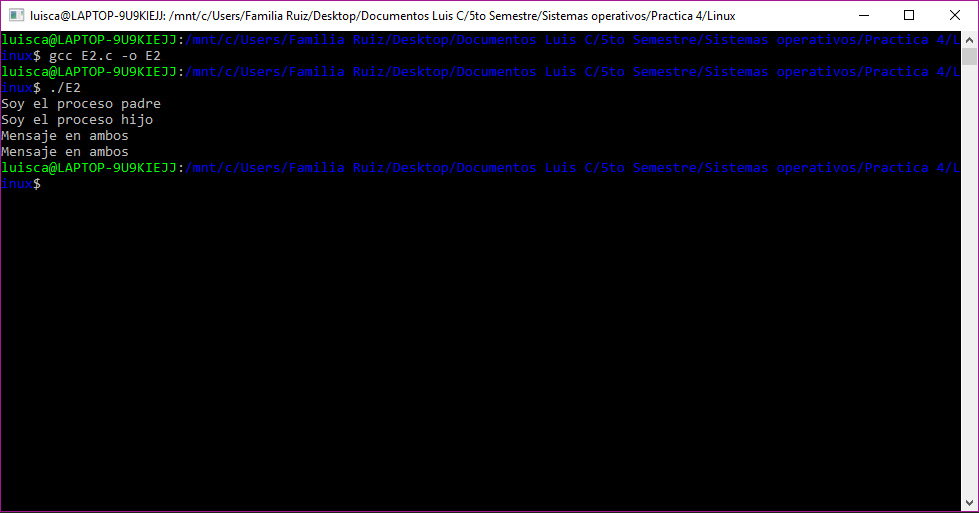
\includegraphics[scale=.5]{Imagenes/Linux/Ejemplo 2.PNG}
            \end{center}
        \newpage
        \item Programe una aplicación que cree el árbol de procesos que se muestra a continuación. \\
        Imagen \\
        Para cada uno de los procesos creados (por copia exacta de código) se imprimirá en pantalla el pid de su padre si se trata de un hijo terminal o los pid’s de sus hijos creados si se trata de un proceso padre.
        
            \begin{center}
                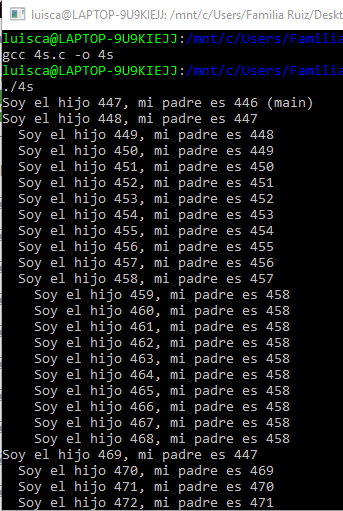
\includegraphics[scale=.6]{Imagenes/Linux/4-1.PNG}
                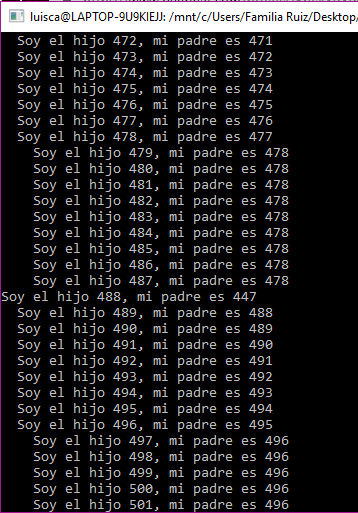
\includegraphics[scale=.6]{Imagenes/Linux/4-2.PNG}
                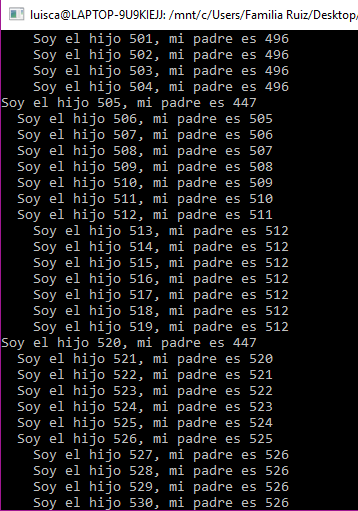
\includegraphics[scale=.6]{Imagenes/Linux/4-3.PNG}
                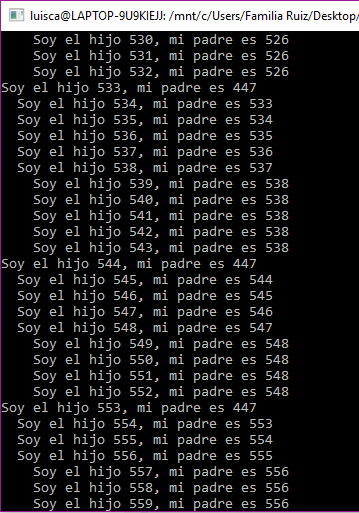
\includegraphics[scale=.6]{Imagenes/Linux/4-4.PNG}
                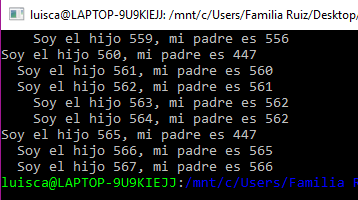
\includegraphics[scale=.6]{Imagenes/Linux/4-5.PNG}
            \end{center}
        \newpage
        A continuación se encuentra el árbol de procesos que se genero:
        
        
        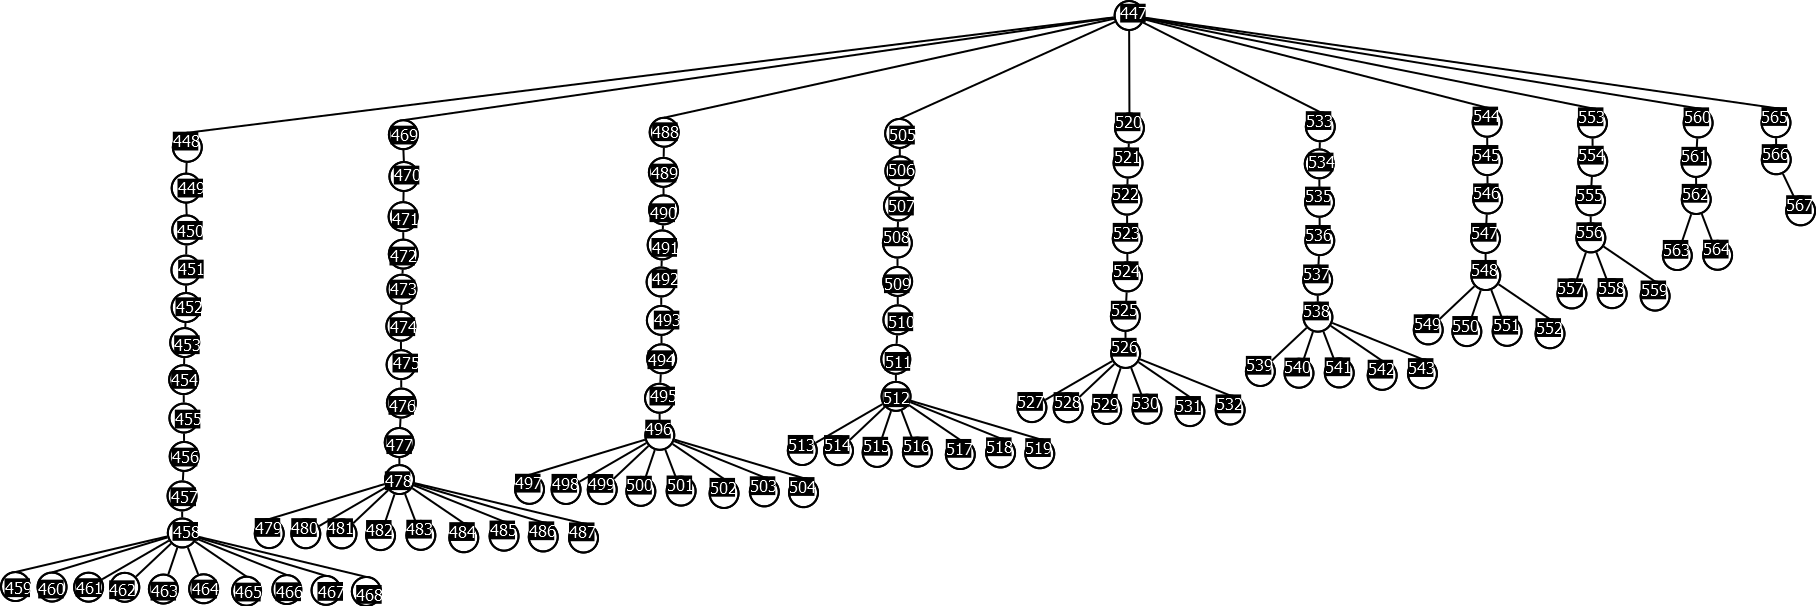
\includegraphics[scale=.26]{Imagenes/Linux/Arbol4.png}
        
        \item Programe una aplicación que cree seis procesos (por copia exacta de código). El primer proceso se encargará de realizar la suma de dos matrices de 10x10 elementos tipo entero, el segundo proceso realizará la resta sobre esas mismas matrices, el tercer proceso realizará la multiplicación de las matrices, el cuarto proceso obtendrá las transpuestas de cada matriz y el quinto obtendrá las matrices inversas.Cada uno de estos procesos escribirá un archivo con los resultados de la operación que realizo.El sexto proceso leerán los archivos de resultados y los mostrará en pantalla cada uno de ellos.\\
        Programe la misma aplicación sin la creación de procesos, es decir de forma secuencial. Obtenga los tiempo de ejecución de las aplicaciones, compare estos tiempos y de sus observaciones.
        \begin{center}
                 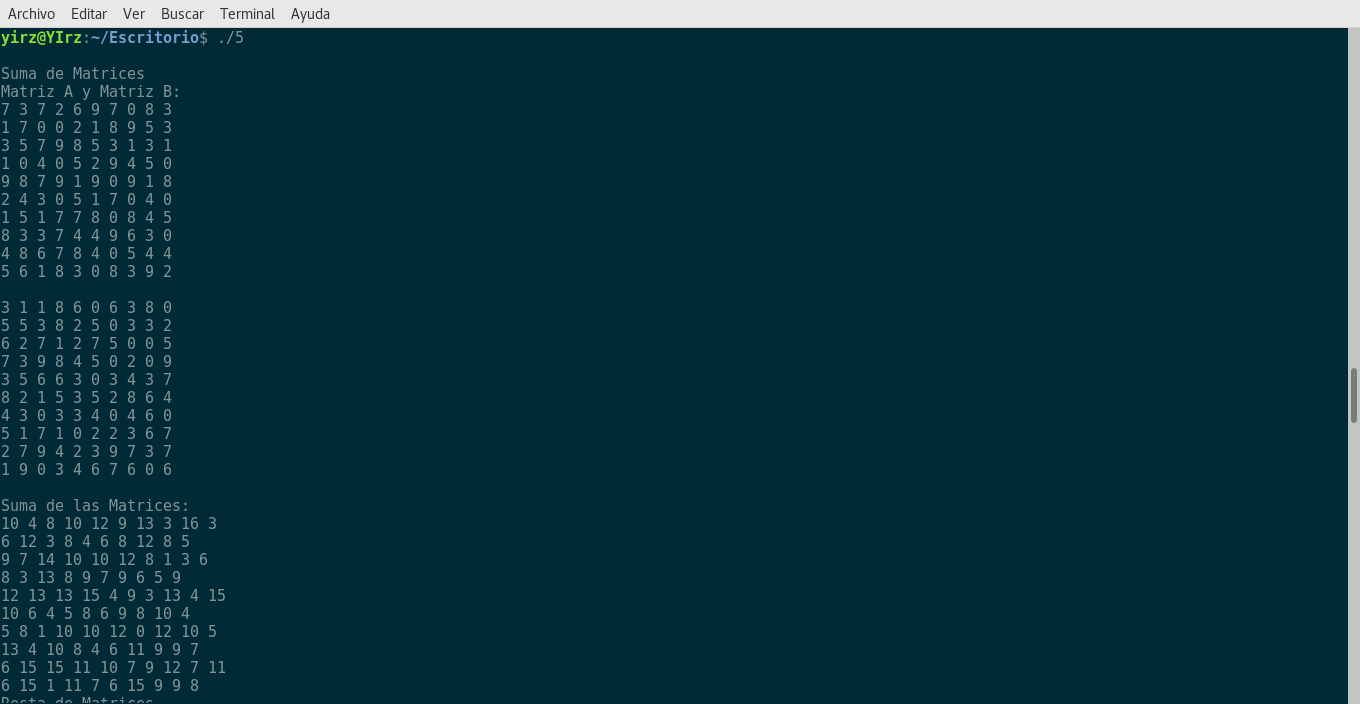
\includegraphics[scale=.35]{Imagenes/Linux/Suma.png}\\
                \end{center}
                 \\
                \begin{center}
                     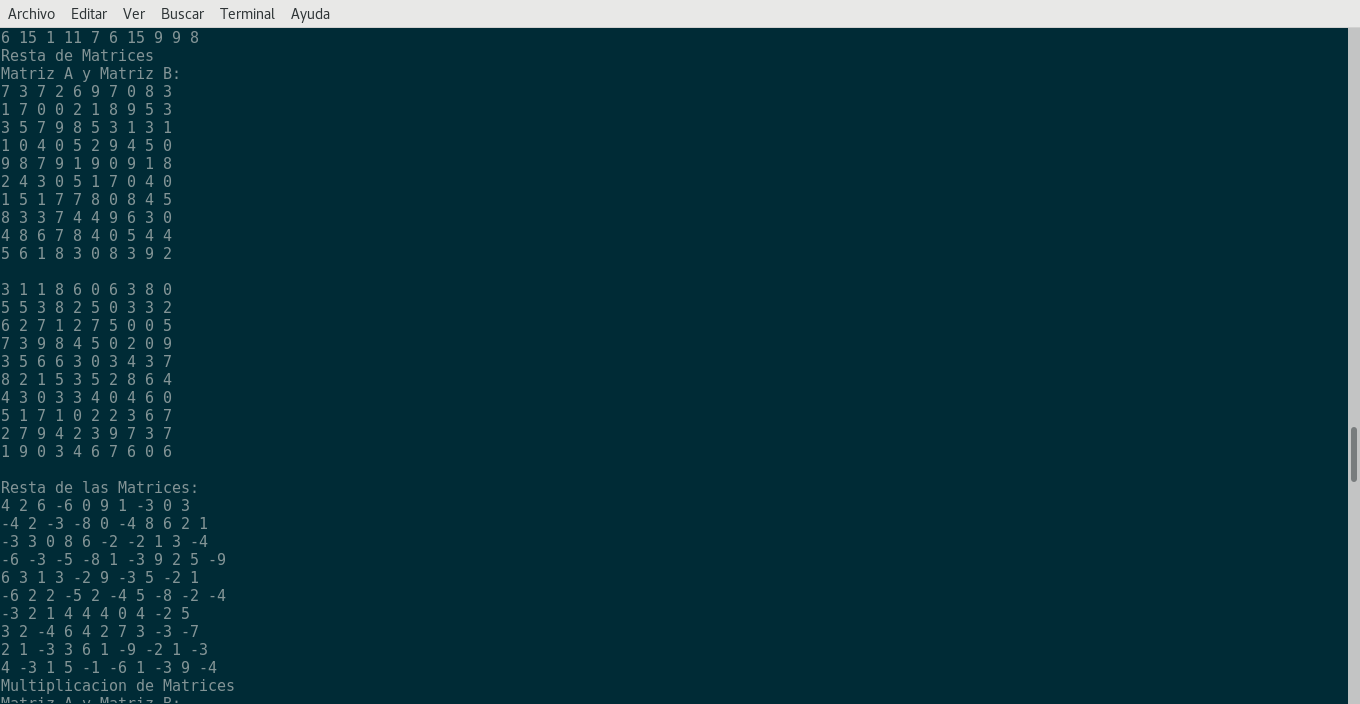
\includegraphics[scale=.35]{Imagenes/Linux/Resta.png}\\
                \end{center}
                \begin{center}
                      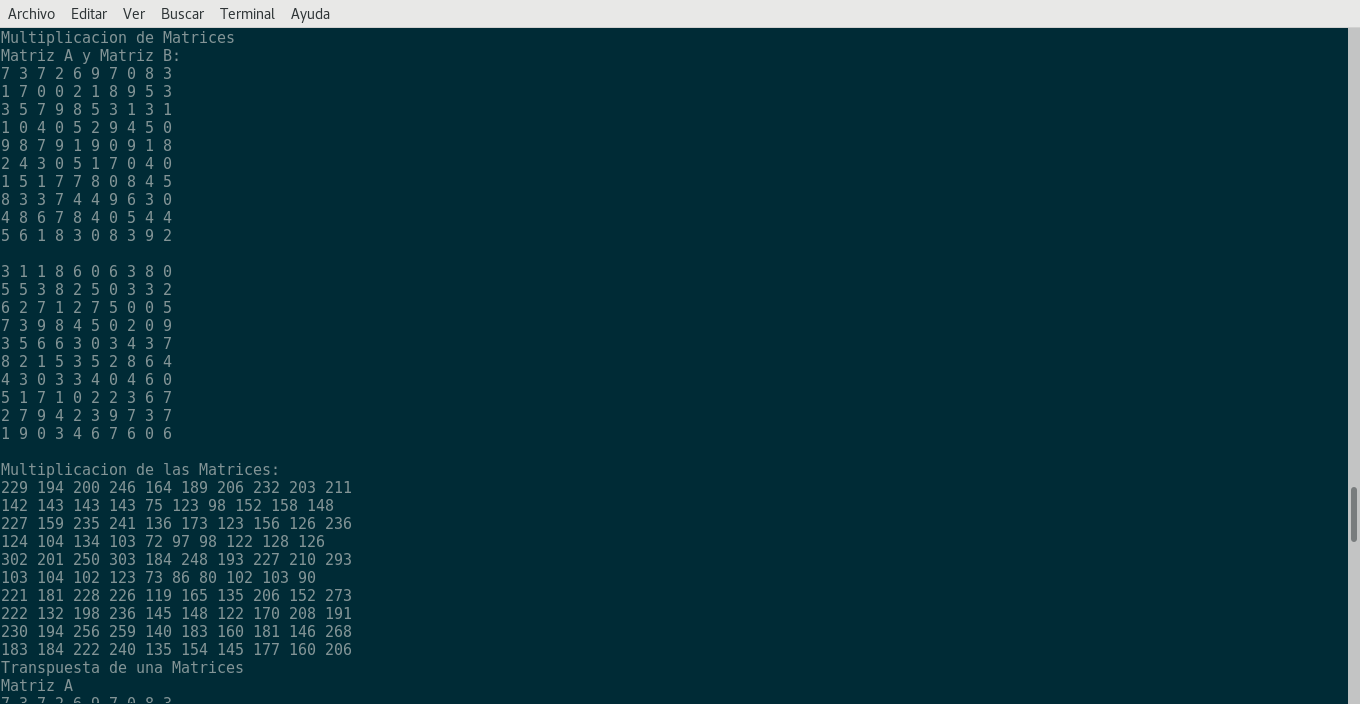
\includegraphics[scale=.35]{Imagenes/Linux/Multiplicacion.png}\\
                \end{center}
                \begin{center}
                    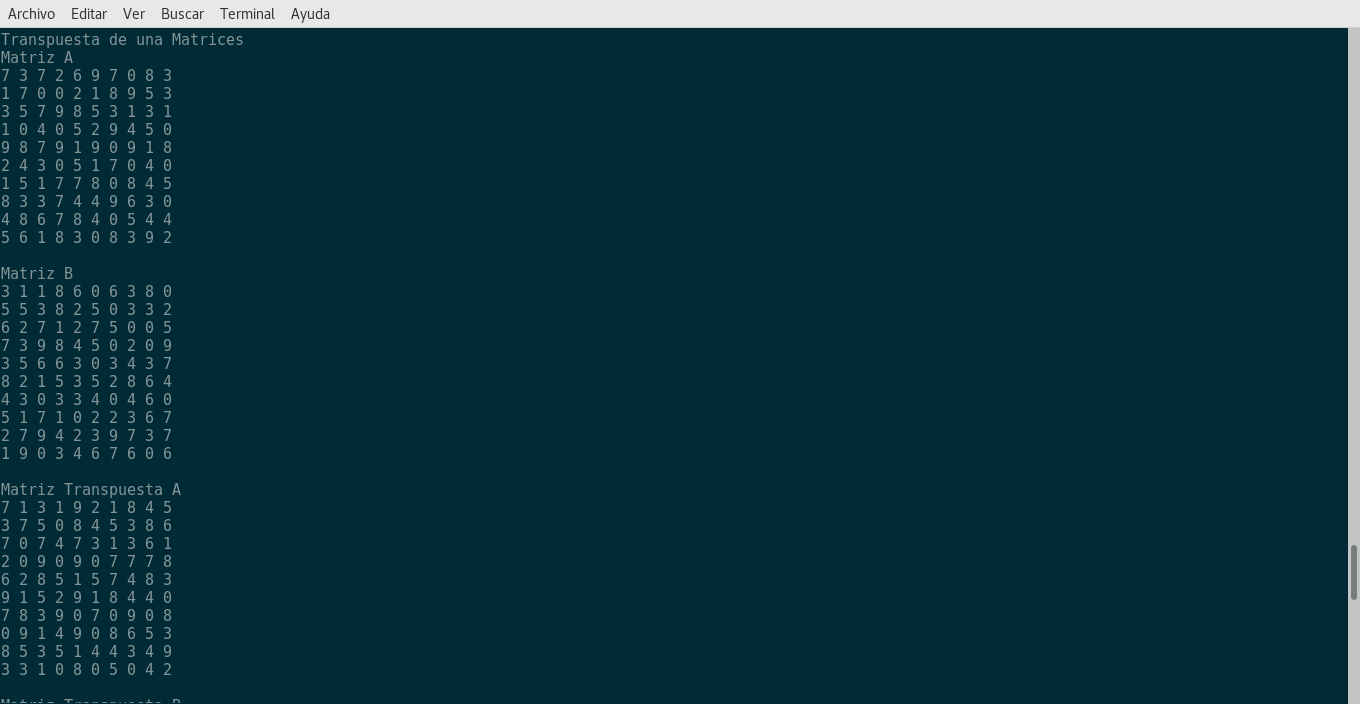
\includegraphics[scale=.35]{Imagenes/Linux/Transpuesta1.pn}
                \end{center}
                \begin{center}
                    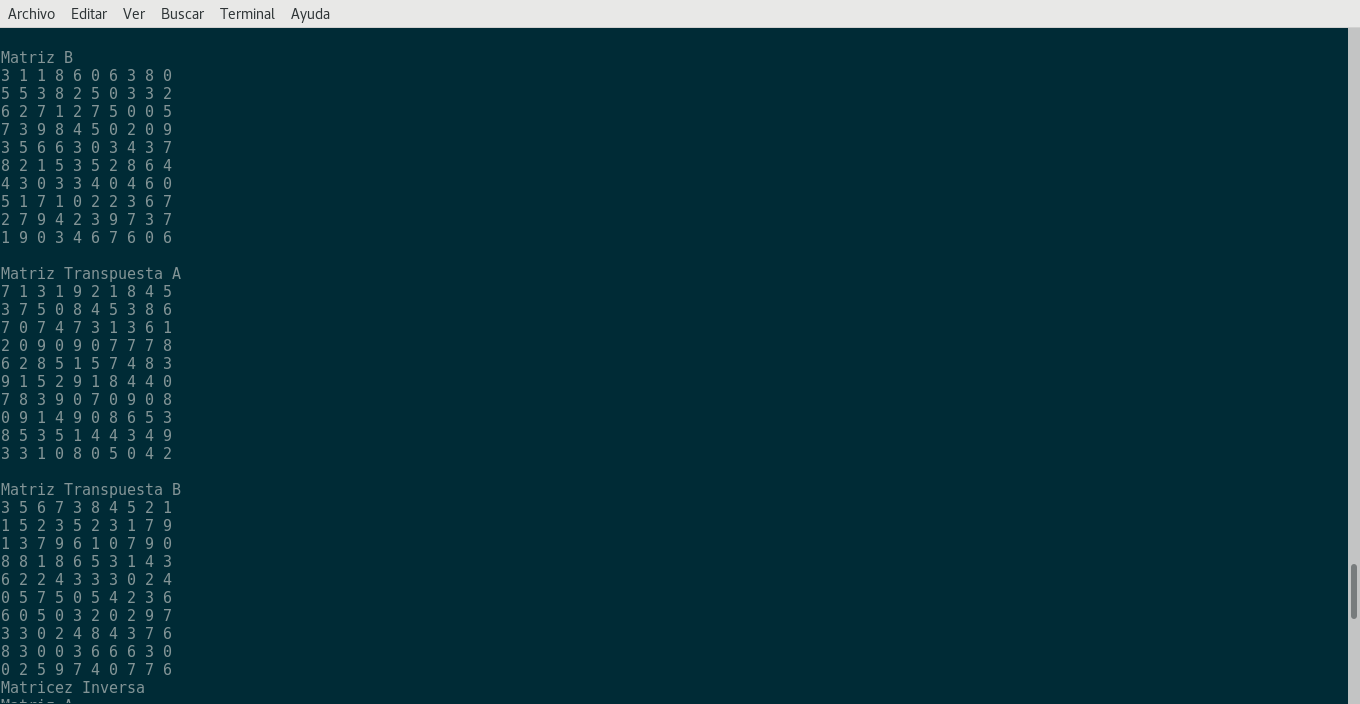
\includegraphics[scale=.35]{Imagenes/Linux/Transpuesta2.png}
                \end{center}  
                \begin{center}
                    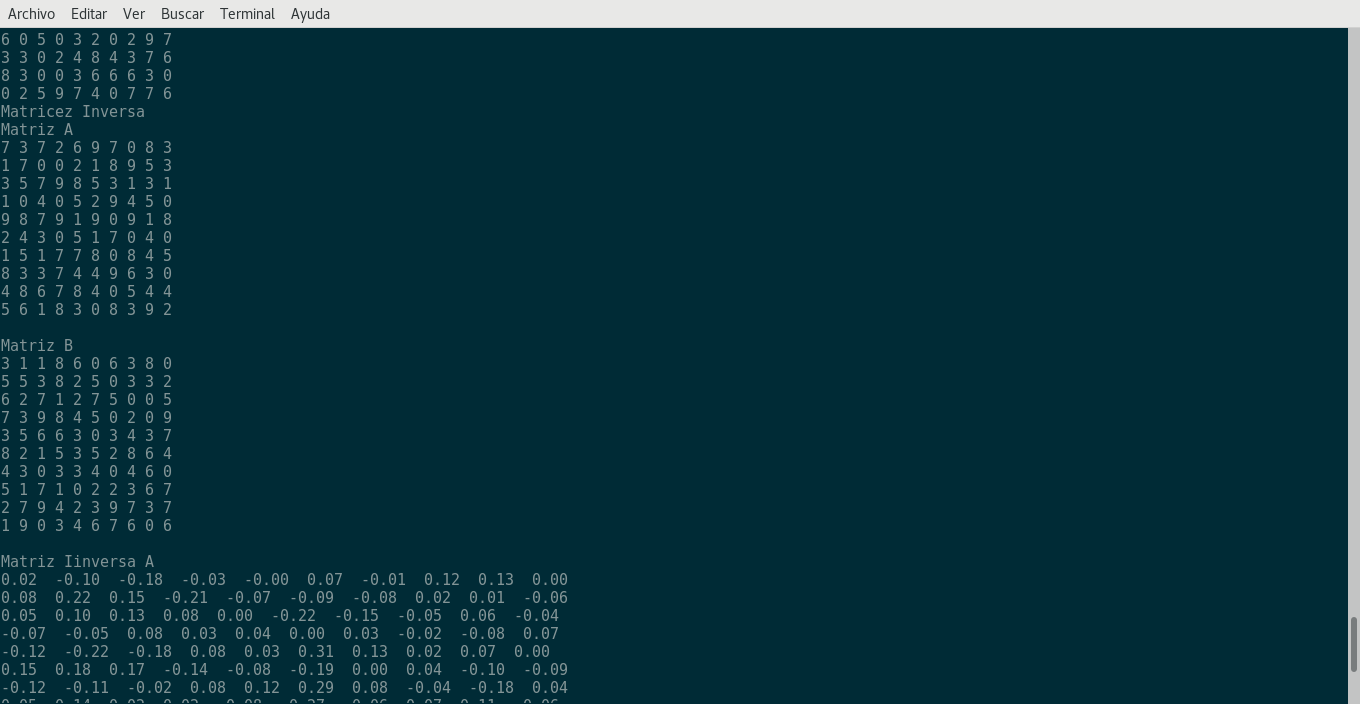
\includegraphics[scale=.35]{Imagenes/Linux/Inversa1.png}\\
                \end{center}
                
                 \begin{center}
                      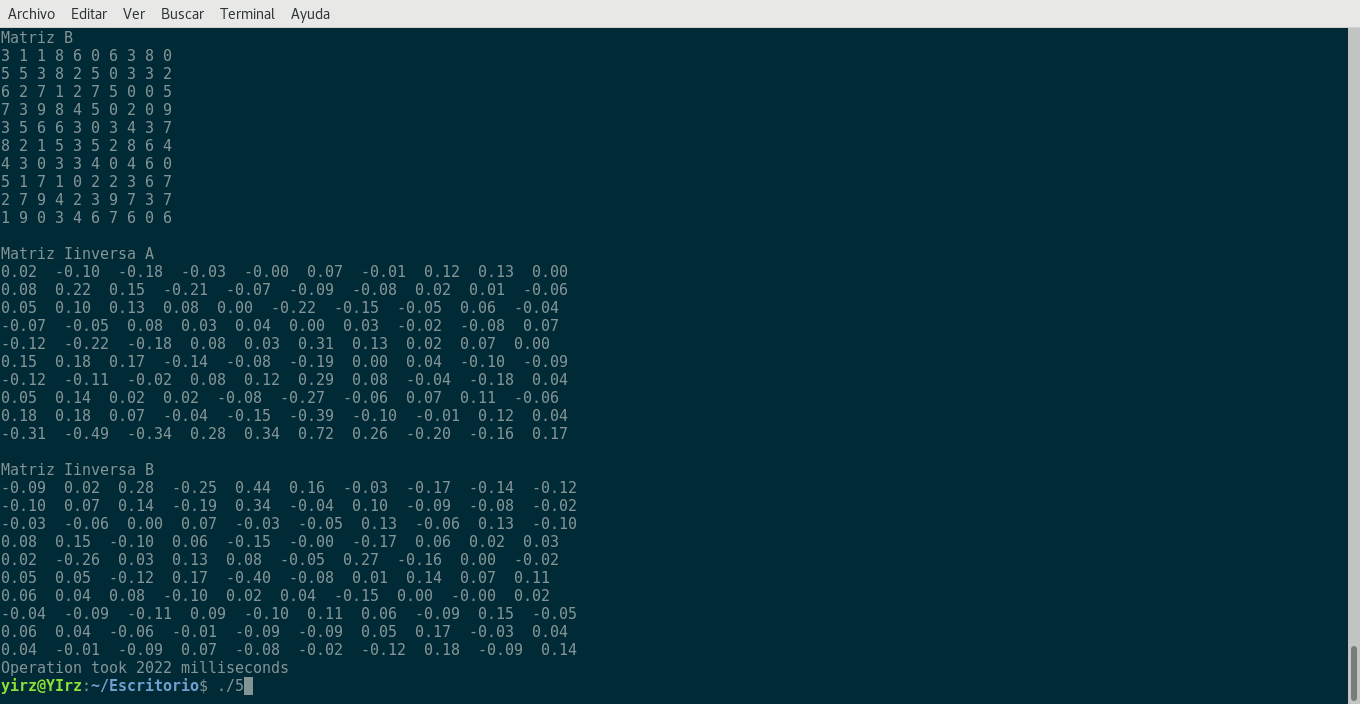
\includegraphics[scale=.35]{Imagenes/Linux/Inversa2.png}
                 \end{center}
                  
                 \begin{center}
                      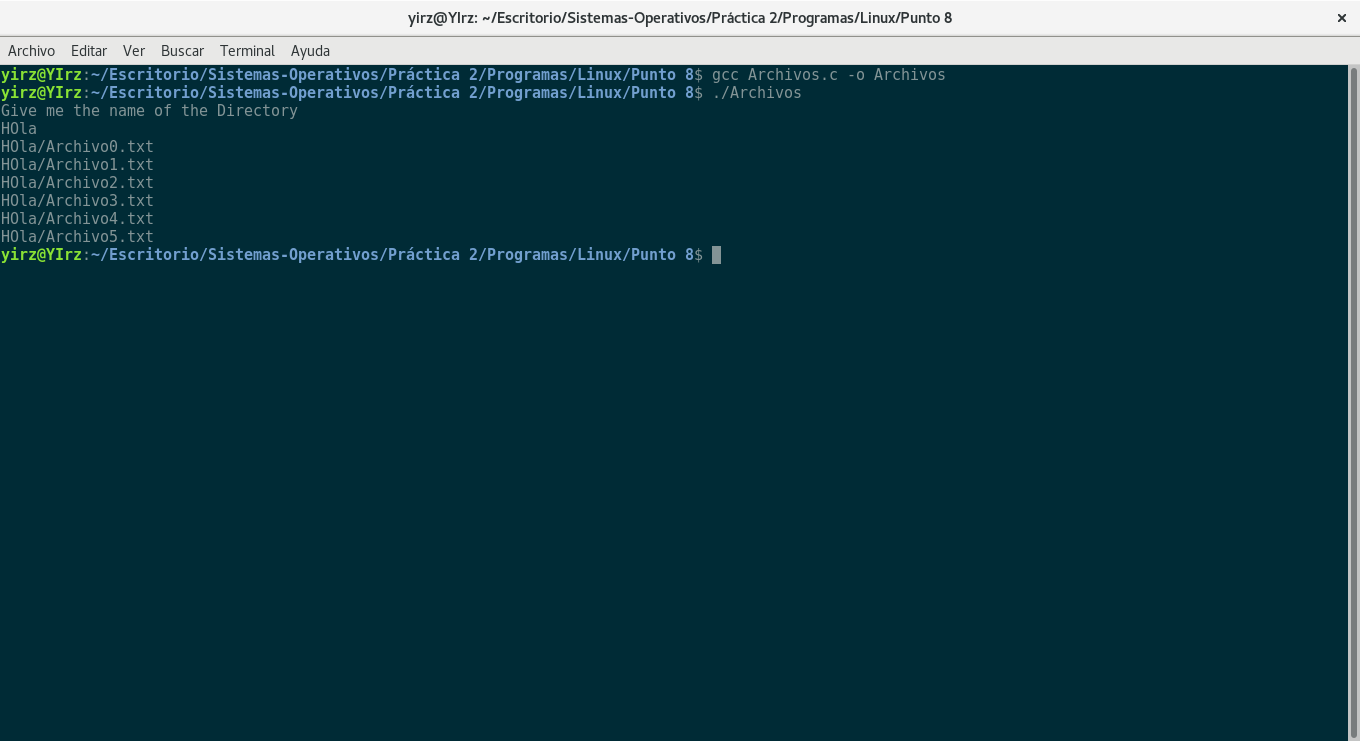
\includegraphics[scale=.35]{Imagenes/Linux/Archivos.png}
                 \end{center}
        \newpage
        \item Capture, compile y ejecute los 2 programas de creación de un nuevo proceso por copia exacta de código que a continuación se muestra. Observe su funcionamiento y experimente con el código.\\

             \textbf{Código 1}
            \lstinputlisting{Codigo/Linux/Padre.c}
            \textbf{Código 2}
            \lstinputlisting{Codigo/Linux/Hijo.c}
            \textbf{Ejemplo por sustitución de código}
            \begin{center}
             \newpage   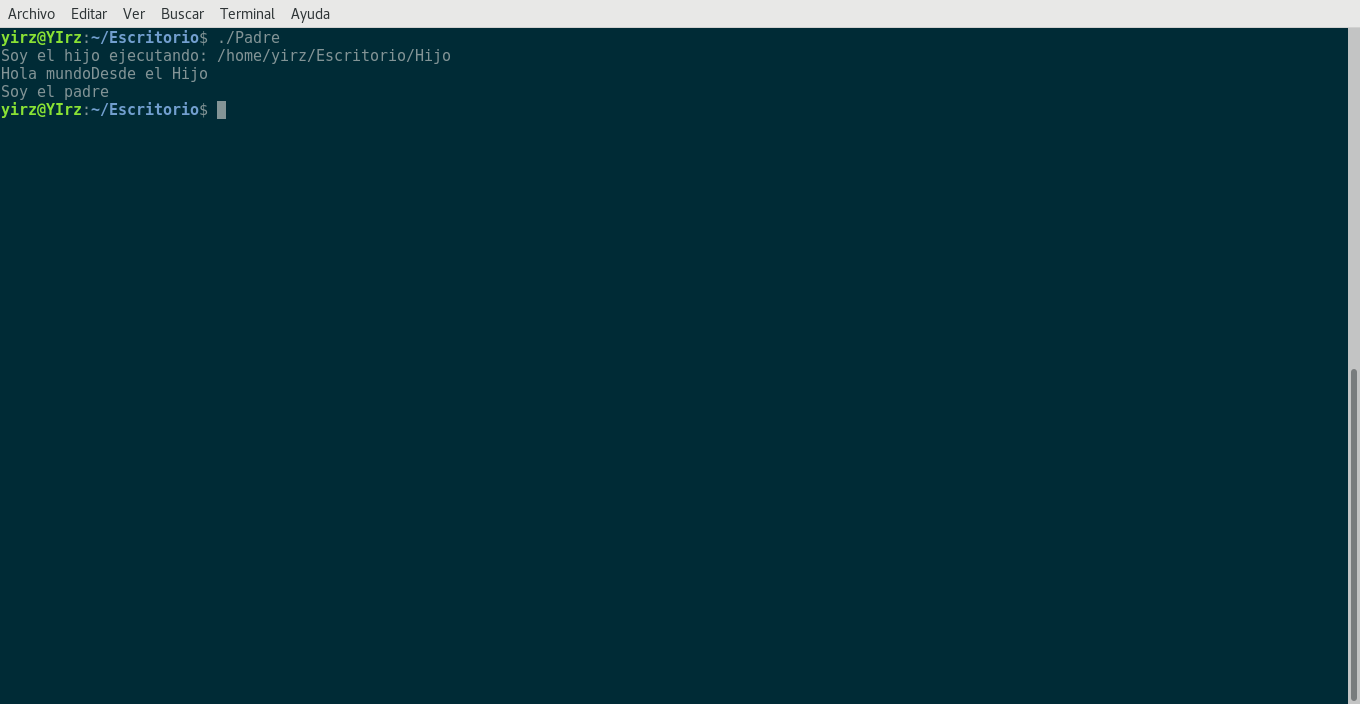
\includegraphics[scale=.35]{Imagenes/Linux/Ejemplo3.png}
            \end{center}
        \item Programe una aplicación que cree un proceso hijo a partir de un proceso padre, el hijo creado a su vez creará tres procesos más. Cada uno de los tres procesos generados ejecutará tres programas diferentes mediante sustitución de código, el primer programa evaluara una expresión aritmética, el segundo programa cambiara los permisos de un archivo dado y el tercer programa obtendrá las matrices inversas que programo anteriormente. Observe el funcionamiento de su programa detalladamente y responda la siguiente pregunta ¿Es posible un funcionamiento 100\% concurrente de su aplicación?
        
        No es posible una aplicación totalmente concurrente debido a que internamente el equipo tiene sus propios planificadores que deciden que programa se ejecutara primero, además de por ejemplo cuando se tiene que recibir algún dato desde teclado, ese programa obtiene los recursos para que se pueda llevar a cabo esa acción, entonces los demás programas tendrán que esperar a que este proceso termine. Además cada proceso requiere una terminal para solicitar entradas. 

        
        \item Programe la aplicación desarrollada en el punto 5 de la sección de Linux utilizando esta vez la creación de procesos por sustitución de código.
        
        \begin{center}
                 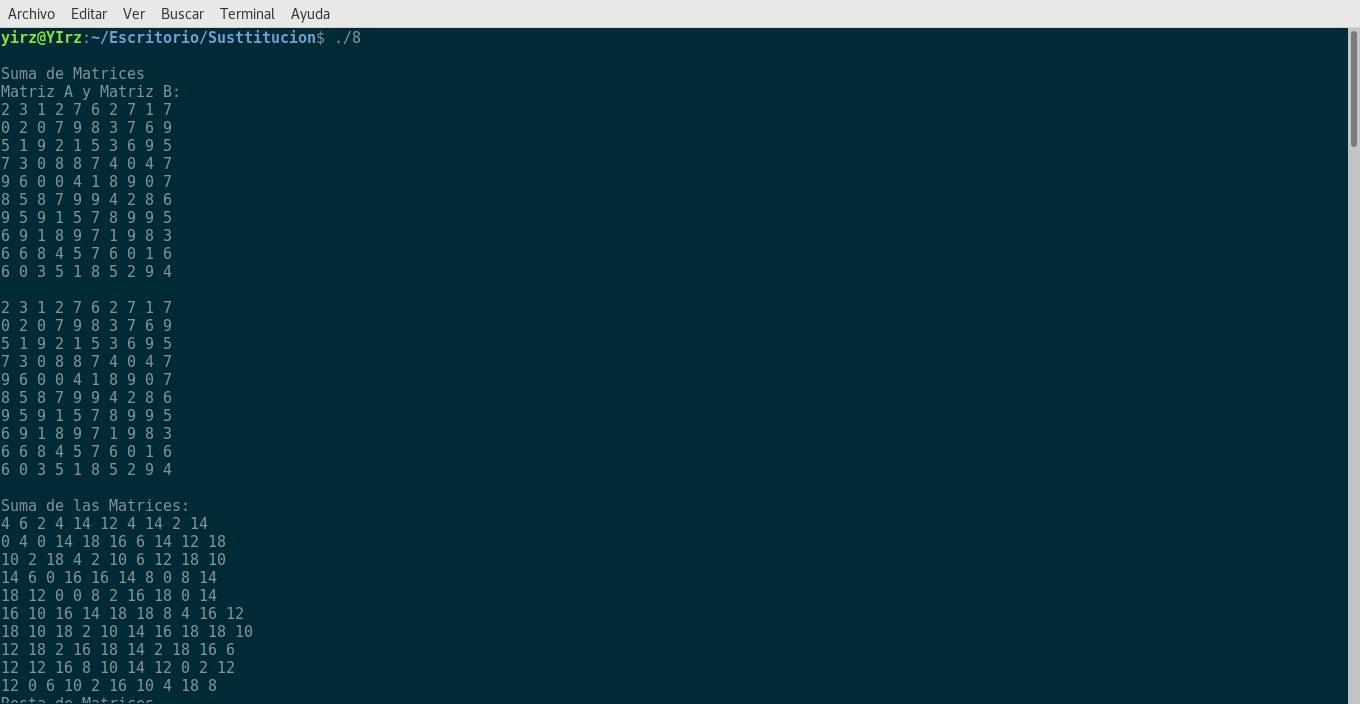
\includegraphics[scale=.35]{Imagenes/Linux/SumaS.png}\\
                \end{center}
                
                \begin{center}
                     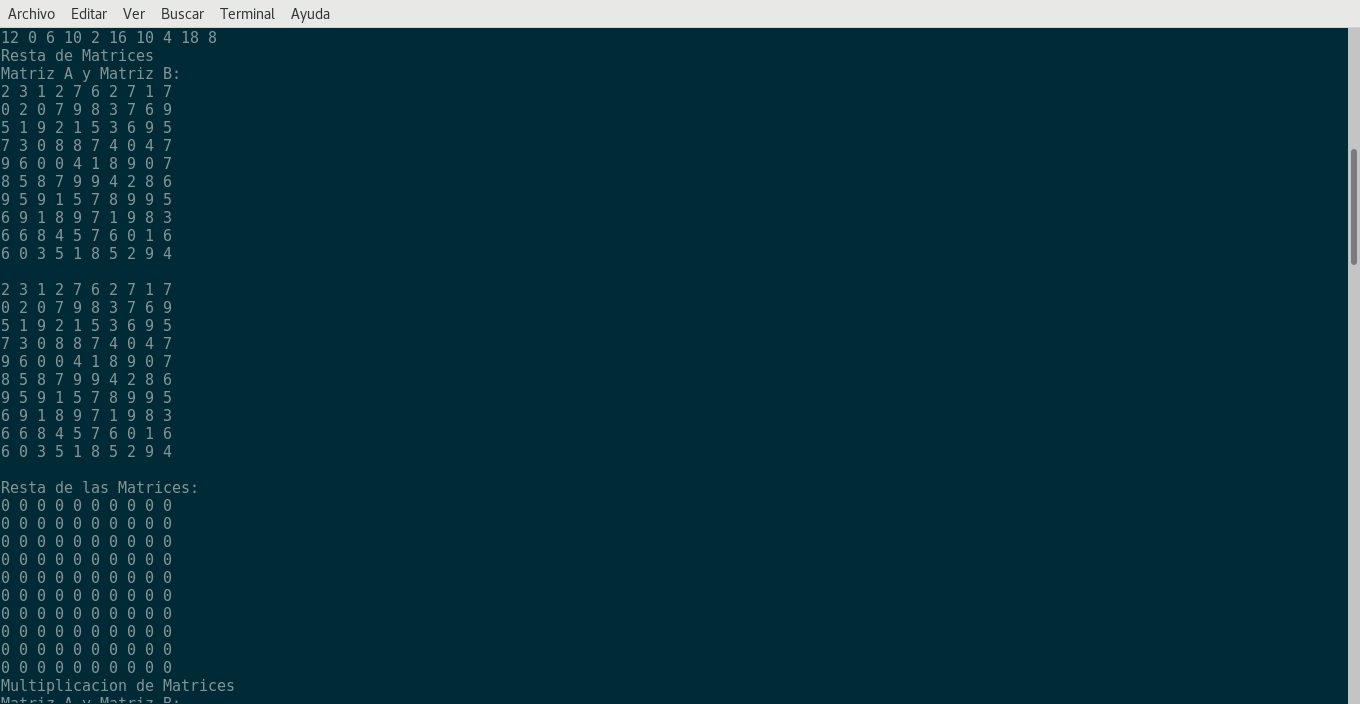
\includegraphics[scale=.35]{Imagenes/Linux/RestaS.png}\\
                \end{center}
                \begin{center}
                      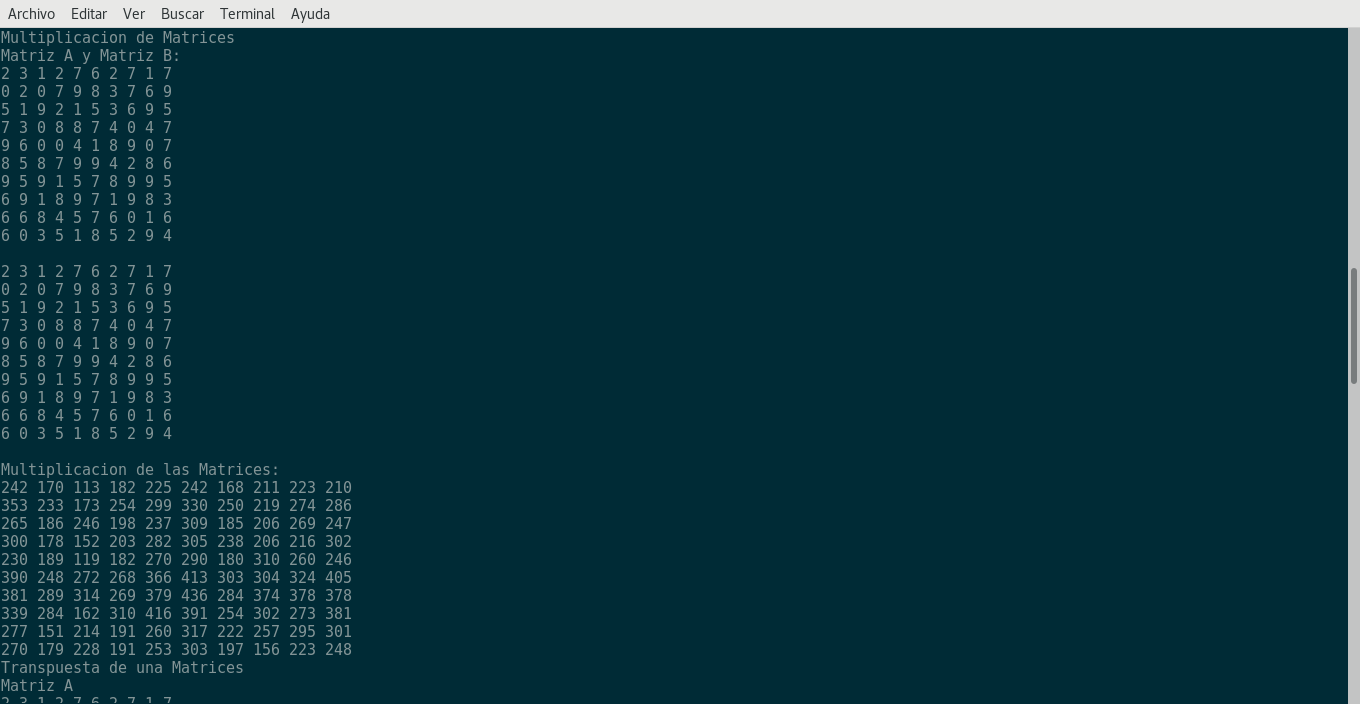
\includegraphics[scale=.35]{Imagenes/Linux/MultiplicacionS.png}\\
                \end{center}
                \begin{center}
                    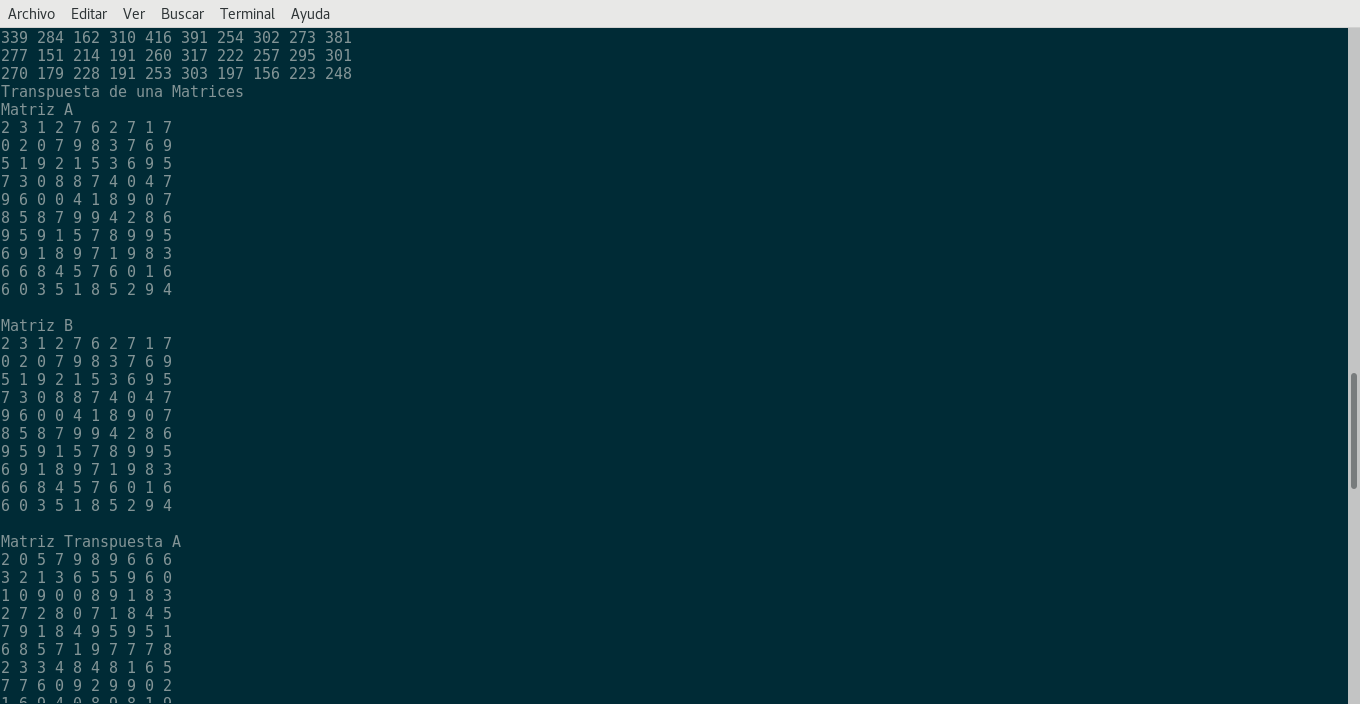
\includegraphics[scale=.35]{Imagenes/Linux/Transpuesta1S.pn}
                \end{center}
                \begin{center}
                    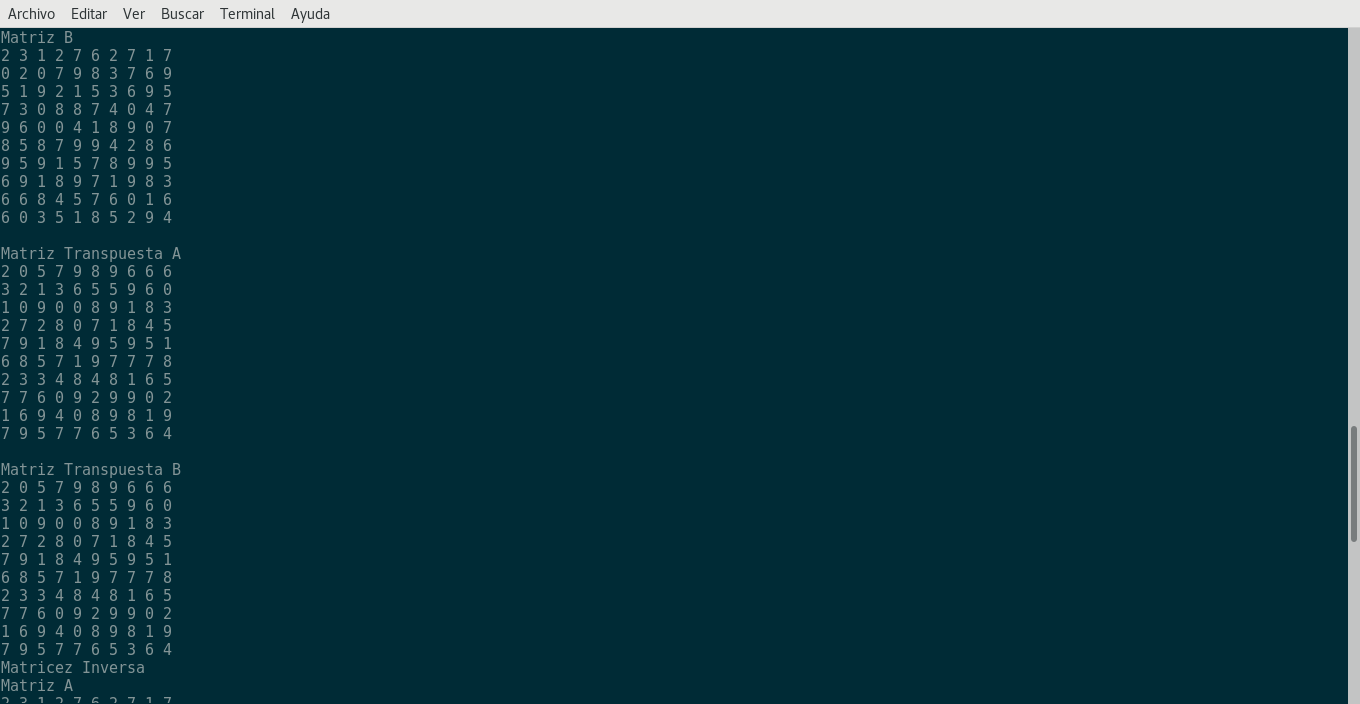
\includegraphics[scale=.35]{Imagenes/Linux/Transpuesta2S.png}
                \end{center}  
                \begin{center}
                    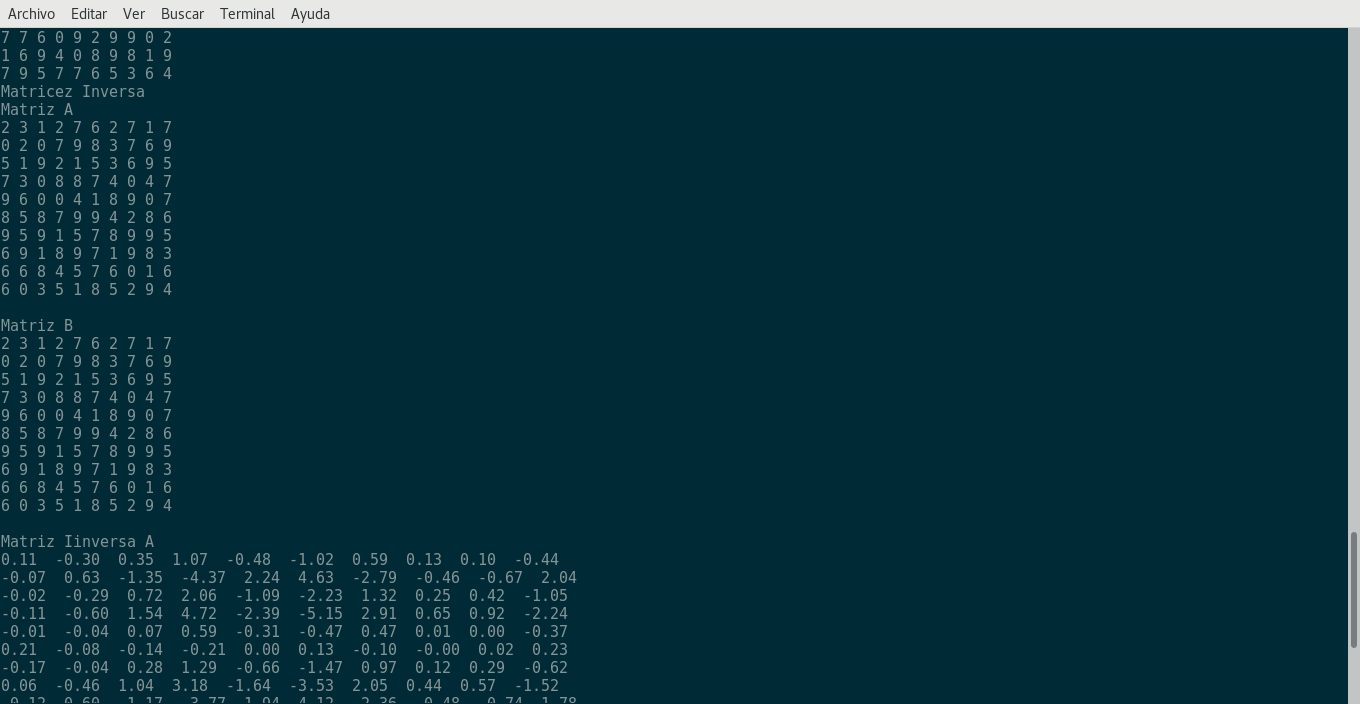
\includegraphics[scale=.35]{Imagenes/Linux/Inversa1S.png}\\
                \end{center}
                
                 \begin{center}
                      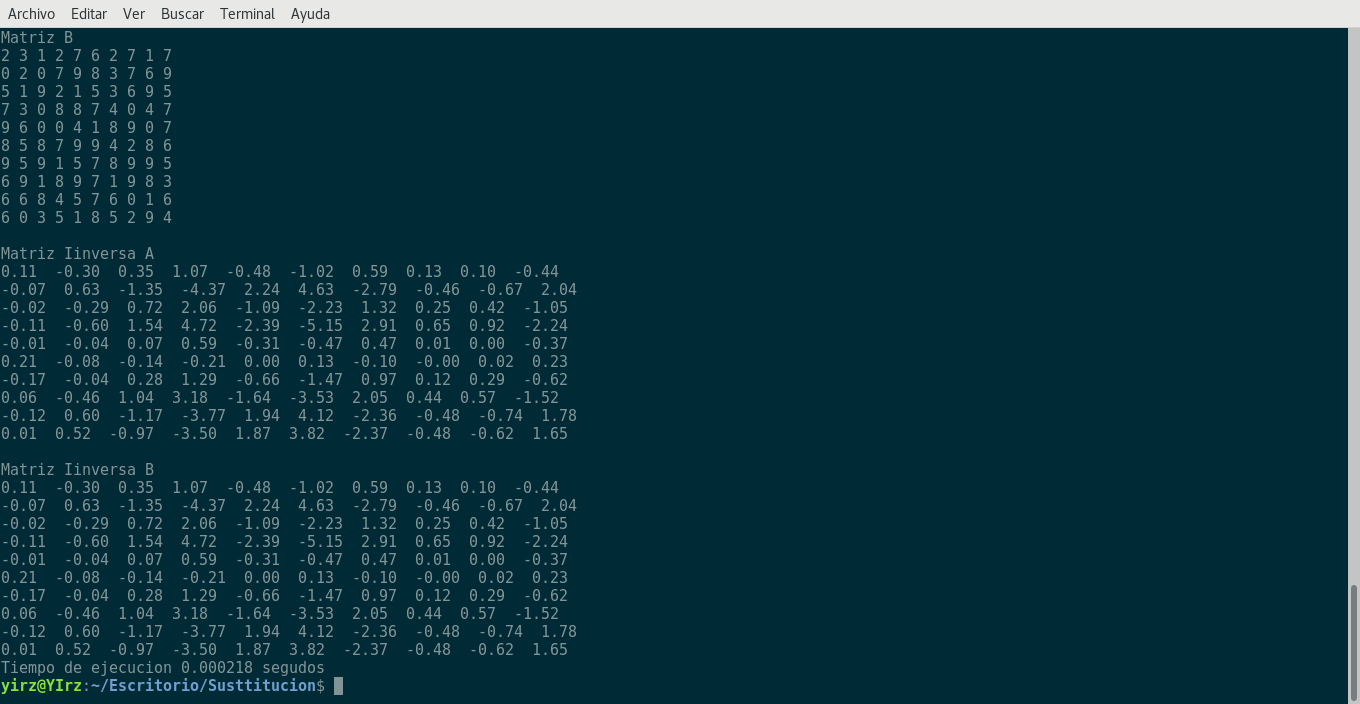
\includegraphics[scale=.35]{Imagenes/Linux/Inversa2S.png}
                 \end{center}
                  
                 \begin{center}
                      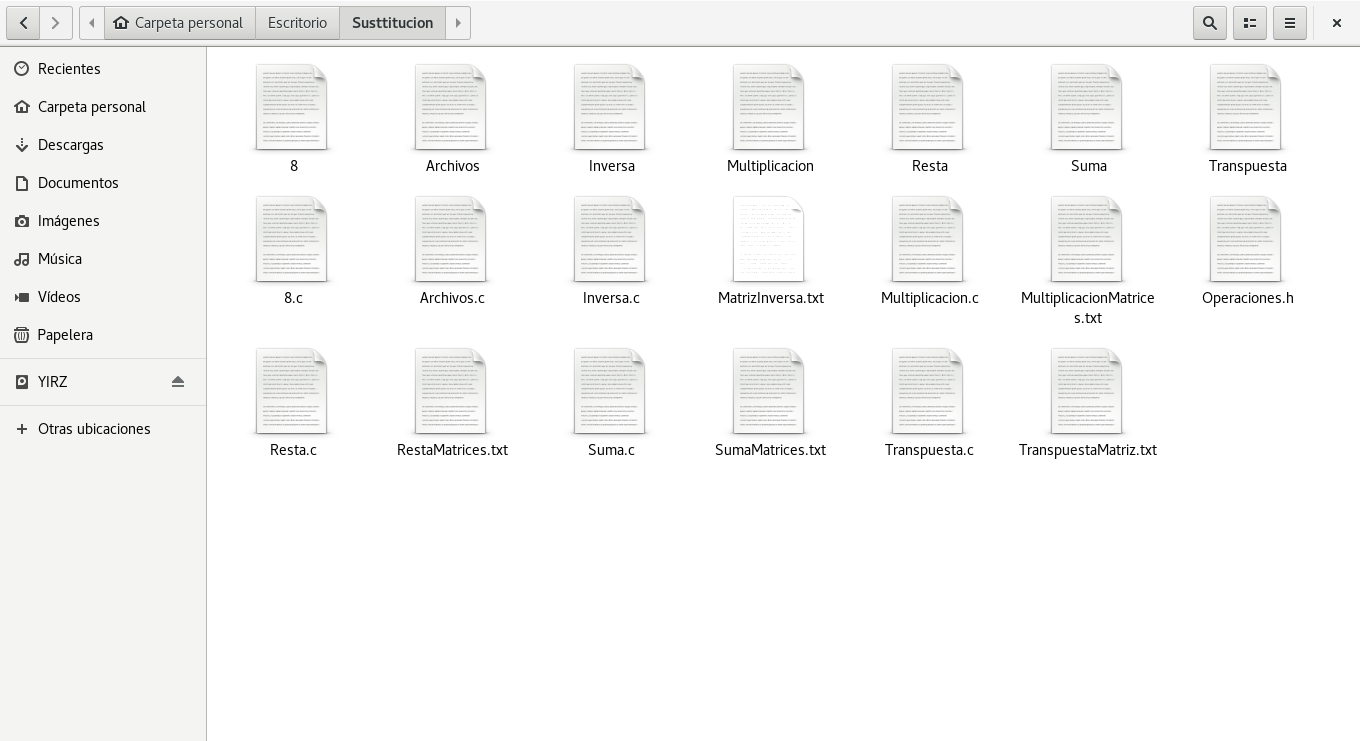
\includegraphics[scale=.35]{Imagenes/Linux/ArchivosS.png}
                 \end{center}
            \item Tiempo (No Concurrente)
                  \begin{center}
                      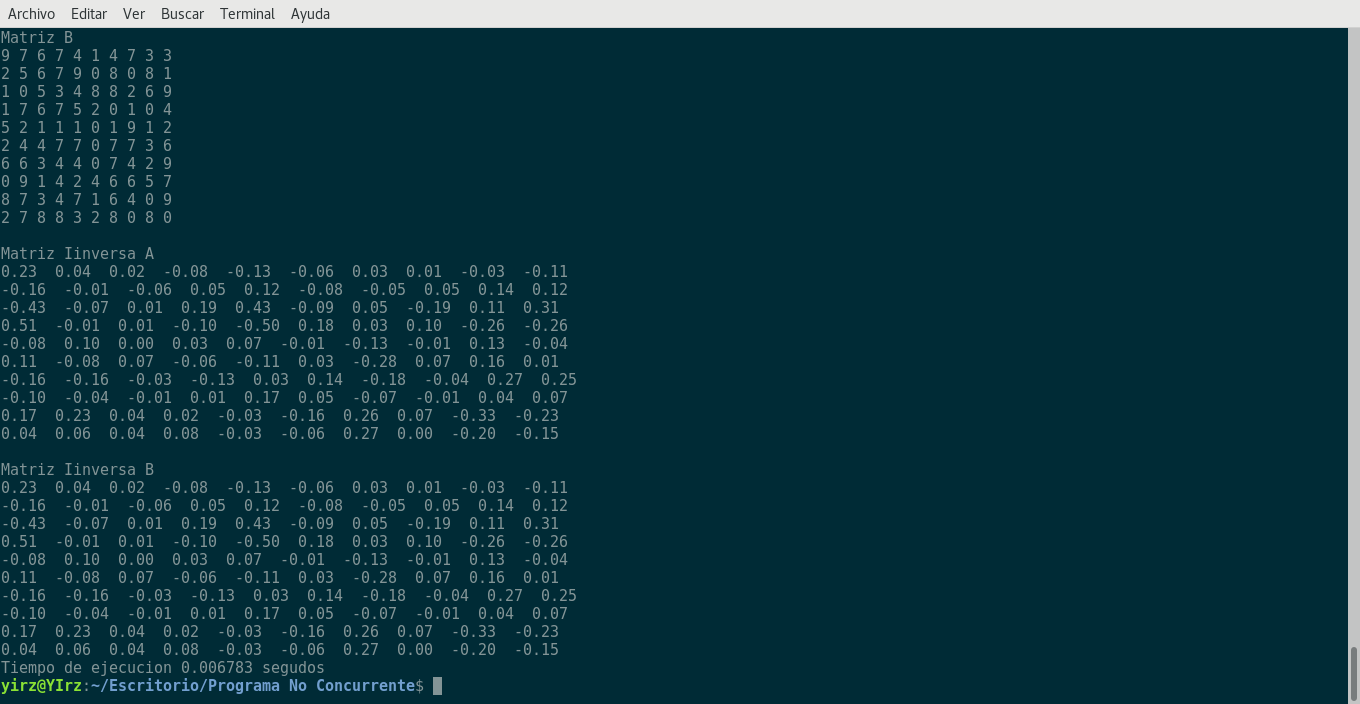
\includegraphics[scale=0.35]{Imagenes/Linux/Tiempo.png}
                 \end{center}
    \end{enumerate}
    
\newpage
\subsection{Windows}
    \begin{enumerate}
        \item Inicie sesión en Windows
        \item Para esta práctica se utilizará el ambiente de programación Dev C/C++
        \item Capture y compile el programa de creación de un nuevos procesos que a continuación se muestra\\
        
            \lstinputlisting{Codigo/Windows/Padre.c}
        \item Capture y compile el programa que contendrá al proceso hijo que a continuación se muestra.
            \lstinputlisting{Codigo/Windows/Hijo.c}
        \newpage
        \item Ejecute el primer código pasando como argumento el nombre del archivo ejecutable del segundo código capturado. Observe el funcionamiento del programa, reporte sus observaciones y experimente con el código
        \begin{center}
            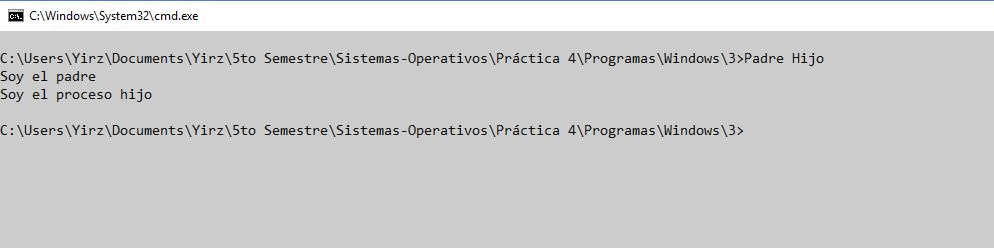
\includegraphics[scale=.5]{Imagenes/Windows/3.JPG}
        \end{center}
        \item Compare y reporte tanto las diferencias como similitudes que encuentra con respecto a la creación de procesos por sustitución de código en Linux. 
        
        \textbf{Consultar Observaciones.}
        
        \item Programe una aplicación que cree un proceso hijo a partir de un proceso padre, el hijo creado a su vez creará 5 procesos hijos más. A su vez cada uno de los cinco procesos creará 3 procesos mas. Cada uno de los procesos creados imprimirá en pantalla su identificador.
        
        
        La función \textbf{GetCurrentProcessId()} Recupera el identificador de proceso del proceso de llamada. Esta función no tiene parámetros. El valor de retorno es el identificador de proceso del proceso de llamada. Hasta que el proceso finaliza, el identificador del proceso identifica de manera única el proceso en todo el sistema.
        \begin{center}
            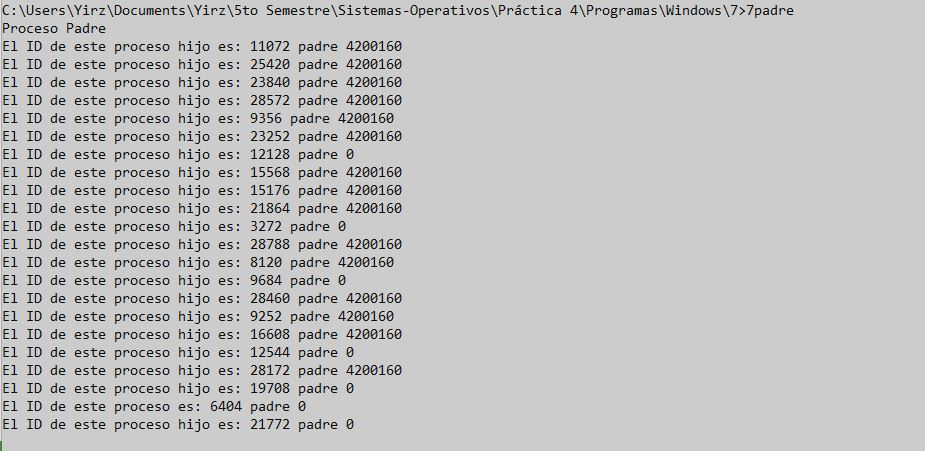
\includegraphics[scale=.5]{Imagenes/Windows/7.JPG}
        \end{center}
        \newpage
        \item Programe la aplicación desarrollada en el punto 5 de la sección de Linux utilizando esta vez la Creación de procesos en Windows.
        
         \begin{center}
                 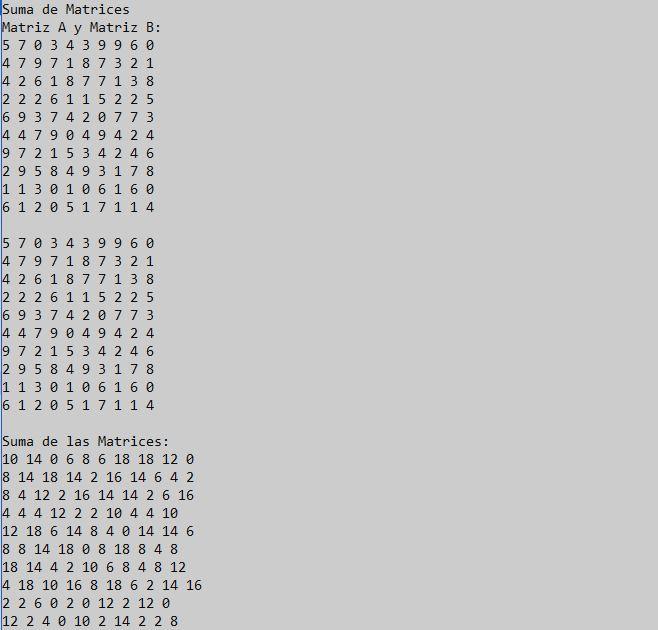
\includegraphics[scale=.5]{Imagenes/Windows/Suma.JPG}\\
                \end{center}
                 
                \begin{center}
                     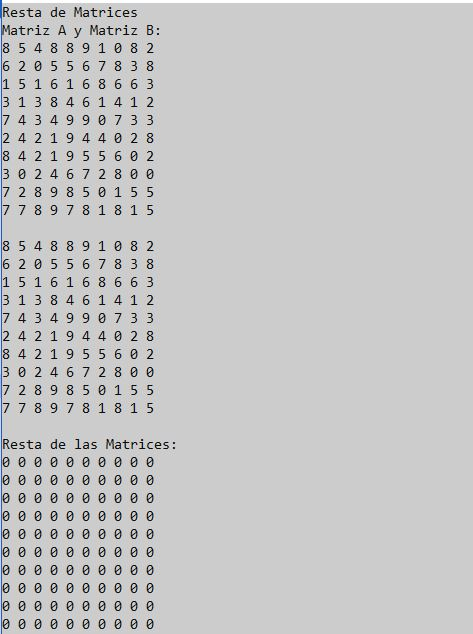
\includegraphics[scale=.5]{Imagenes/Windows/Resta.JPG}\\
                \end{center}
                \begin{center}
                      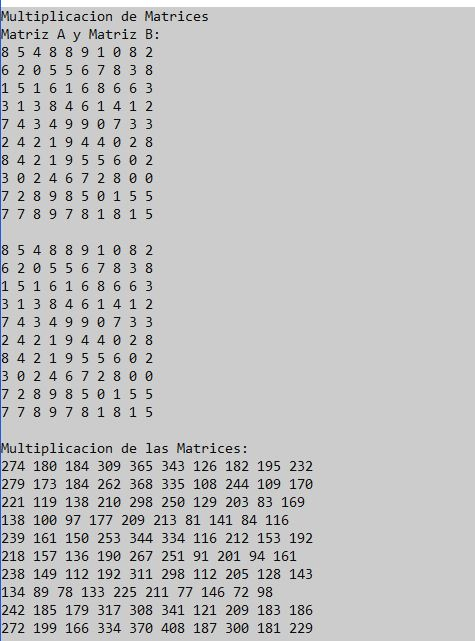
\includegraphics[scale=.5]{Imagenes/Windows/Multiplicacion.JPG}\\
                \end{center}
                \begin{center}
                    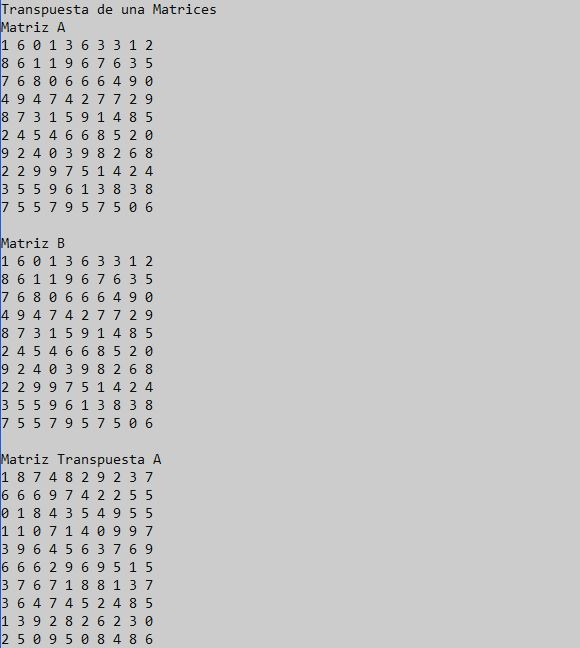
\includegraphics[scale=.65]{Imagenes/Windows/Transpuesta1.JPG}
                \end{center}
                \begin{center}
                    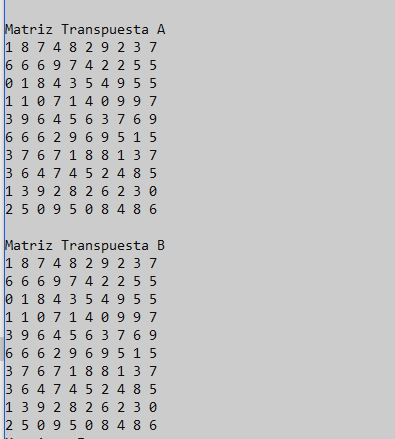
\includegraphics[scale=.65]{Imagenes/Windows/Transpuesta2.JPG}
                \end{center}  
                \begin{center}
                    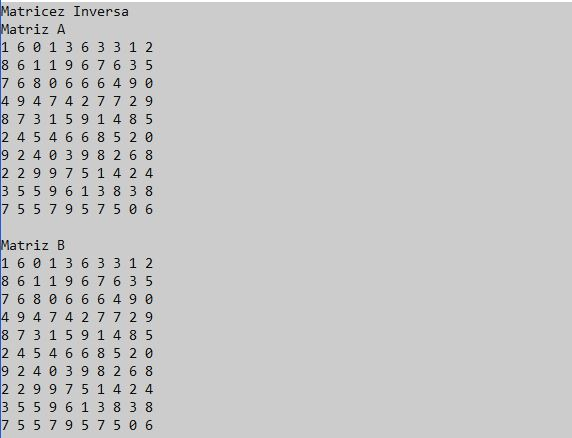
\includegraphics[scale=.65]{Imagenes/Windows/Inversa1.JPG}\\
                \end{center}
                
                 \begin{center}
                      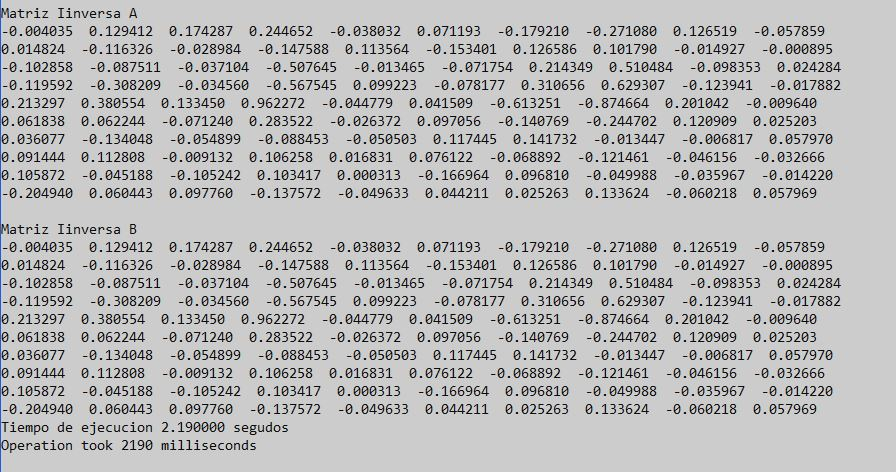
\includegraphics[scale=.55]{Imagenes/Windows/Inversa2.JPG}
                 \end{center}
                  
                 \begin{center}
                      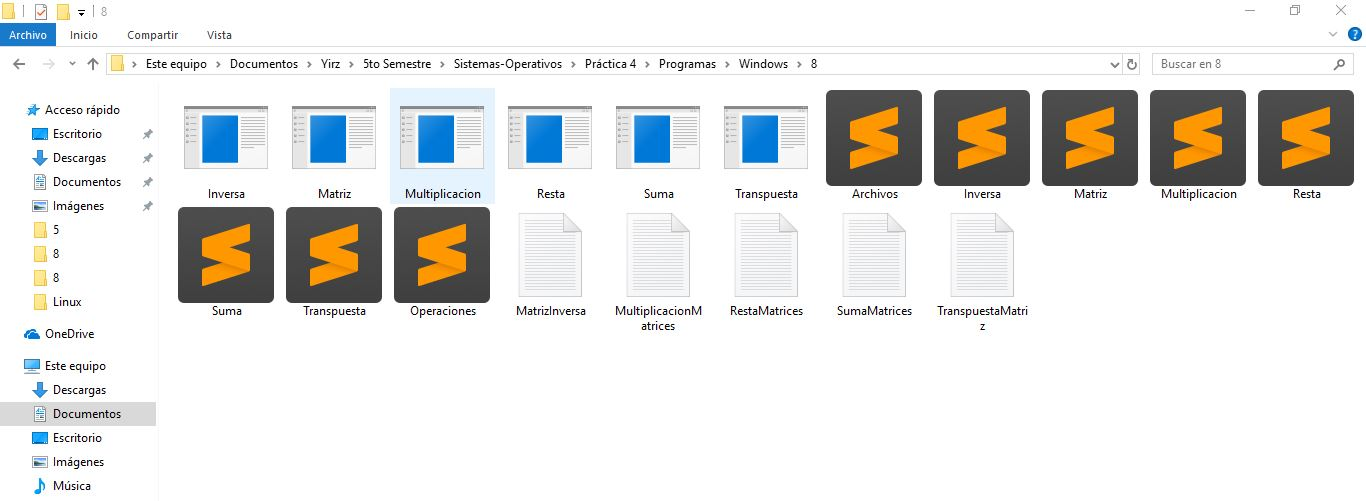
\includegraphics[scale=.45]{Imagenes/Windows/Archivos.JPG}
                 \end{center}
                 \item Tiempo (No Concurrente)
                  \begin{center}
                      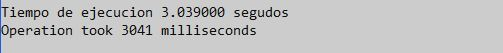
\includegraphics[scale=.7]{Imagenes/Windows/Tiempo.JPG}
                 \end{center}
    \end{enumerate}    

    \subsection{Código Fuente.}
          \subsubsection{Linux}
          \begin{itemize}
                \item \textbf{Punto 4}
                
                \lstinputlisting{Codigo/Linux/4s.c}
                
                \item \textbf{Punto 5}\\
                 \textbf{Operaciones con Matrices}
                 \lstinputlisting{Codigo/Linux/Operaciones.h}
                 \textbf{Creacion de procesos}
                  \lstinputlisting{Codigo/Linux/5.c}
                \item \textbf{Punto 7}
                \lstinputlisting{Codigo/Linux/main.c}
                \item \textbf{Punto 8}\\
                Se utilizo las mismas operaciones mostradas en el \textbf{Punto 5}\\
                \textbf{Creacion de procesos}
                \lstinputlisting{Codigo/Linux/8.c}
                \textbf{Suma}
                 \lstinputlisting{Codigo/Linux/Suma.c}
                \textbf{Resta}
                 \lstinputlisting{Codigo/Linux/Resta.c}
                \textbf{Multipicación}
                  \lstinputlisting{Codigo/Linux/Multiplicacion.c}
                \textbf{Matriz transpuesta}
                  \lstinputlisting{Codigo/Linux/Transpuesta.c}
                \textbf{Matriz Inversa}
                  \lstinputlisting{Codigo/Linux/Inversa.c}
                \textbf{Lectura de Archivos}
                  \lstinputlisting{Codigo/Linux/Archivos.c}
                \textbf{Programa concurrente}
                \lstinputlisting{Codigo/NoConcurrente.c}
          \end{itemize}
    \newpage
    \subsubsection{Windows}
        \begin{itemize}
             \item \textbf{Punto 7}
              \lstinputlisting{Codigo/Windows/7padre.c}
                \lstinputlisting{Codigo/Windows/H1.c}
                \lstinputlisting{Codigo/Windows/H2.c}
                \lstinputlisting{Codigo/Windows/H4.c}
                
              \item \textbf{Punto 8}\\
              \textbf{Operaciones con Matrices}
                 \lstinputlisting{Codigo/Linux/Operaciones.h}
                 \textbf{Creacion de procesos}
                \lstinputlisting{Codigo/Windows/Matriz.c}
                 \textbf{Suma}
                 \lstinputlisting{Codigo/Linux/Suma.c}
                \textbf{Resta}
                 \lstinputlisting{Codigo/Linux/Resta.c}
                 \newpage
                \textbf{Multipicación}
                  \lstinputlisting{Codigo/Linux/Multiplicacion.c}
                  \newpage
                \textbf{Matriz transpuesta}
                  \lstinputlisting{Codigo/Linux/Transpuesta.c}
                \textbf{Matriz Inversa}
                  \lstinputlisting{Codigo/Linux/Inversa.c}
                
        \end{itemize}
            
    
    \newpage
\section{Observaciones.}
Se tienen las siguientes observaciones: 
\begin{itemize}
    \item La ejecución de varios procesos procede a la concurrencia y asignar tiempos a cada uno, lo que agiliza el tiempo de ejecución de cada uno de ellos, dedicando tiempos congruentes a cada uno, que a diferencia de la programación secuencial , ahorra tiempo de ejecución.
    \item La ejecución de procesos en cada uno de los sistemas operativos es diferente en gran proporción, ya que según el sistema operativo es el tipo de creación de procesos, mientras Linux soporta ambas formas de creación, y su combinación, Windows solo soporta la creación de procesos por sustitución de código lo que implicada asociar a cada procesos un procesos ligero.
    \item Los árboles de procesos en un sistema operativo y en el desarrollo de aplicaciones concurrentes, permite organizar mediante una estructura jerárquica, la cual establece relaciones padre - hijo entre los proceso, lo que hace posible heredar ciertos recursos de los procesos padre a sus procesos hijos según sus necesidades de ejecución. 
\end{itemize}


\section{Análisis Crítico.}
    
En cuanto a velocidades  se pude analizar, que la versión programación concurrente tiene la capacidad de ser mas rápido al momento de la ejecución que en la programación secuencial, por ejemplo en el programa concurrente de operaciones con matrices el tiempo de ejecución fue de 2022 milisegundos mientras que en la versión secuencial fue de 0.006783 segundos, el tiempo de ejecución concurrete de creación de procesos por sustitución de código fue de 0.000218 segundos, por lo tanto la ejecución más rápida fue por creación de procesos por copia exacta de código. Sin embargo la concurrencia no se logra en su totalidad, es necesario tomar en cuenta las necesidades de ejecución de cada proceso y los recursos que este requiere según el objetivo que cumpla el programa.

\newpage
\section{Conclusiones.}

Finalmente, en está primera práctica sobre la revisión del administrador de procesos en los sistemas operativos de Linux y Windows, se pudo corroborar que, los procesos son un elemento principal de este administrador. Durante la presente práctica, se revisaron procesos creados por petición de aplicación en sus dos formas: creación de procesos por copia exacta de código y por sustitución de código. 

La creación de procesos por copia exacta de código permite la concurrencia, que es una propiedad de los sistemas en la cual los procesos de un cómputo se hacen simultáneamente, y pueden interactuar entre ellos, sin embargo, no se puede lograr un concurrencia totalmente dicha, puesto que los programas que se ejecutan simultáneamente, mantienen recursos compartidos, así que dependiendo de la ejecución de cada uno y los recursos que ocupe será el nivel de logro de la concurrencia. 

Por otro lado, mediante la presente práctica se corroboraron los problemas que genera la destrucción de un proceso en la creación de procesos por sustitución de código y se comprobó la solución propuesta de combinar ambas formas de creación, creando un proceso hijo a partir de un proceso padre, por copia exacta de código y posteriormente realizar la creación de procesos por sustitución de código.


\end{document}

